\chapter{Реализация системы}
\label{ch:chap3}

\section{Предпосылки разрабатываемой системы}
Nav2 является отличной основой для реализации автономной навигации для мобильных роботов. 

Однако, если сравнивать функциональные возможности данного ПО с предлагаемой архитектурой автономной системы, представленной на Рисунке \ref*{fig:sense_think_act}, то можно увидеть, что в Nav2 отсутствует компонент системного контроля. \\
Отсутствие компоненты системного контроля приводит к ограниченному набору обстоятельств, в которых робот может надежно выполнять навигацию. Одна из основных проблем, с которой сталкиваются мобильные роботы - создание надежного представления среды. Непредвиденные события могут серьезно ограничить надежность представления среды. \\
Примерами таких событий, которые в настоящее время не обрабатываются должным образом, являются проскальзывание колес, изменение ориентации под воздействием внешних факторов или необнаруживаемые препятствия. Такие ситуации провоцируют небезопасное поведение и требуют вмешательства человека-оператора и восстановления работоспособности робота вручную.

Также для навигации в динамическом окружении в системе Nav2 отсутствуют компоненты учета динамических объектов для более безопасного функционирования вблизи людей и других агентов. Об актуальности данной проблемы говорит то, что в рамках программы Summer of Code 2021, участником предлагалась задача по разработке решения динамического обнаружения препятствий для Nav2 на основе 2D LIDAR \cite{nav2-challenge}.  

Итак, для успешной навигации в динамическом окружении в разрабатываемую систему требуются внести следующие изменения:
\begin{enumerate}
    \item Увеличение степени автономности - так как среда является динамической, то возможность доступа оператора к роботу уменьшается и является важным уменьшить степень вовлеченности оператора при работе робота
    \item Слежение за важными узлами робота и возможность быстро реагировать на критические ситуации - робот должен гарантировать безопасность объектов в окружении, поэтому требуется определять ситуации (например, поломка LIDAR) при которых робот теряет возможность безопасного функционирования
    \item Планирование пути с учетом динамических объектов - требуется изменить систему навигации для учета динамических объектов
\end{enumerate}

Требуемая система принятия решений разрабатывалась с учетом пунктов выше.

\section{Стандартная архитектура для навигации}
В качестве основы была взята стандартная архитектура для решения задач навигации при использовании ROS2. Архитектура состоит из следующих компонент:
\begin{itemize}
    \item Nav2 - набор пакетов для навигации;
    \item Turtlebot3 - модель мобильного робота;
    \item AMCL - пакет для локализации робота в 2D, осован на методе Монте-Карло;
    \item SLAM Toolbox - пакет для задачи SLAM, используется для изначального картирования местности;
    \item Map server - пакет для выполнения операций с построенными картами местностей (сохранение, загрузка, редактирование).
\end{itemize}

\begin{figure}[h]
    \centering
    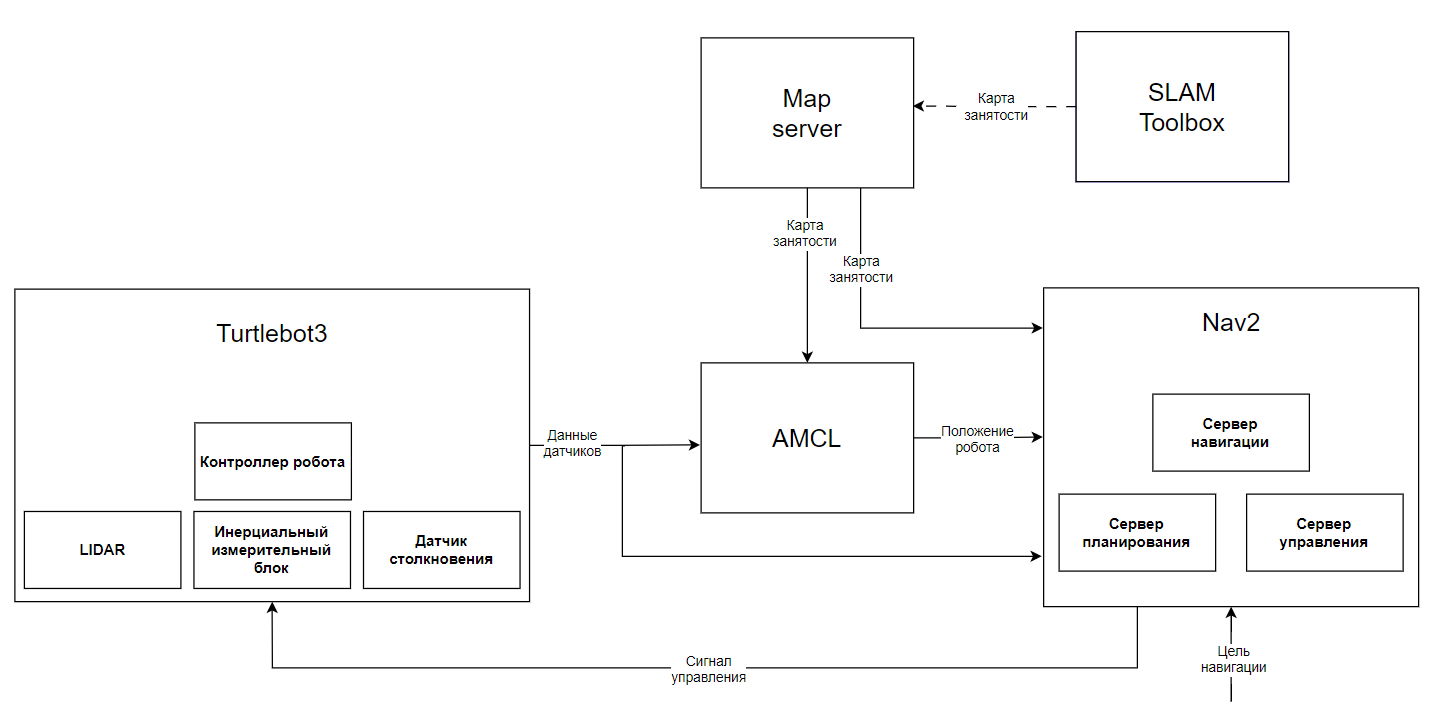
\includegraphics[width=1.0\textwidth]{images/chap_3/sys_arch_nav2.png}
    \caption{Архитектура стандартной системы навигации Nav2}
    \label{fig:sys_arch_nav2}
\end{figure}

\section{Компоненты разработанной системы принятия решений}
Разработанная система принятия решений включает в себя две подсистемы:
\begin{enumerate}
    \item Система контроля - выполняет задачу контроля за функционированием робота. В основе системы - поведенческое дерево, которое позволяет переключать различные поведения в соответствии с принципами модульности, иерархичности, реактивности и наглядности. Система котроля анализирует следующее:
    \begin{enumerate}
        \item Состояние датчика LIDAR;
        \item Состояние датчика IMU;
        \item Состояние одометрии;
        \item Уровень заряда батареи;
        \item Состояние планировщика траектории;
        \item Столкновения с объектами;
        \item Ориентация в пространстве.
    \end{enumerate}
    \item Система учета динамических объектов - выполняет задачи:
    \begin{enumerate}
        \item Разделение объектов на карте местности на статические и динамические
        \item Слежение за обнаруженными динамическими объектами и оценка их скоростей
        \item Добавление области стоимости для динамических объектов на карту стоимости
    \end{enumerate}
\end{enumerate}

\begin{figure}[h]
    \centering
    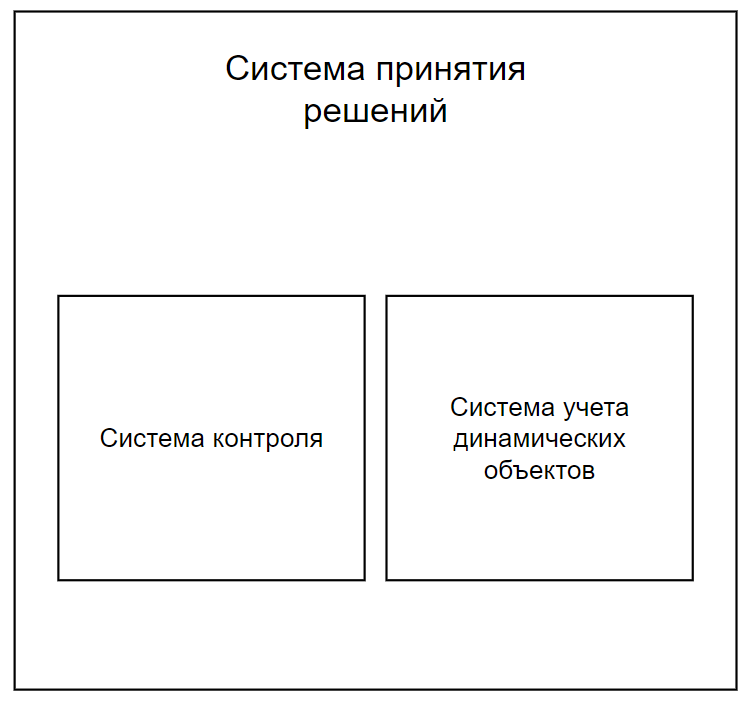
\includegraphics[width=0.5\textwidth]{images/chap_3/dms.png}
    \caption{Компоненты разработанной системы принятия решений}
    \label{fig:dms}
\end{figure}

\section{Структура программной реализации системы}

Для удобства проектирования исходного кода системы были созданы четыре рабочих пространства (рабочее пространство - это каталог, содержащий пакеты ROS2):
\begin{itemize}
    \item \textit{tb3\_ws} - рабочее пространство, содержащее пакеты описывающие модель робота Turtlebot3, позволяющие выполнять Nav2 на роботе, а также проводить симуляцию в Gazebo. Данные пакеты были скачены и собраны с \cite{tb3-git} для того чтобы была возможность модификации исходных файлов
    \item \textit{nav2\_ws} - рабочее пространсвтво для пакетов Nav2. Аналогично пакетам из \textit{tb3\_ws}, были скачены и собраны с \cite{nav2-git} для дальнешего внесения изменений 
    \item \textit{supervisory\_sys\_ws} - рабочее пространство для реализации системы контроля робота
    \item \textit{dyn\_obs\_avoid\_sys\_ws} - рабочее пространство для реализации системы учета динамических объектов
\end{itemize}

\section{Система контроля}

\subsection{Архитектура системы}

\begin{figure}[h]
    \centering
    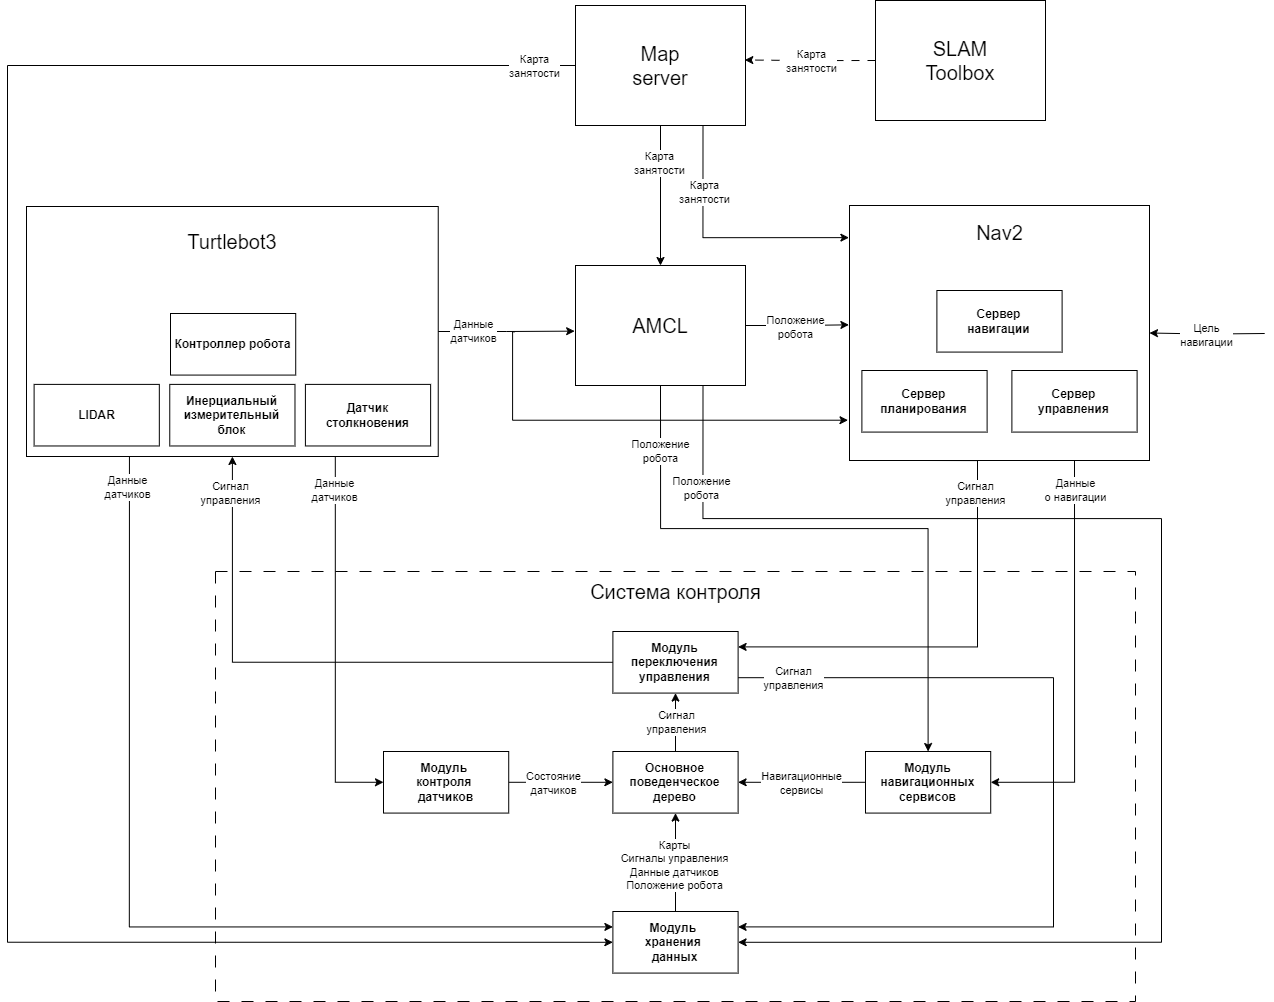
\includegraphics[width=1.0\textwidth]{images/chap_3/supervisory_system.png}
    \caption{Архитектура системы контроля}
    \label{fig:supervisory_system}
\end{figure}

На Рисунке \ref*{fig:supervisory_system} изображена архитектура стандартной системы навигации с внедрением разработанной система контроля. \\
Система контроля включает 5 ключевых модулей, каждый из которых реализован в качестве отдельного ROS пакета. Описание каждой компоненты приведено ниже в соответствующих пунктах.

\subsection{Модуль контроля датчиков}

Данный модуль подписывается на темы (topics) \textit{/odom, /imu, /scan}, из которых получает данные с сенсоров. Если сообщения перестают поступать, то модуль определяет это и обновляет свое внутреннее состояние, записывая информацию о том, что определенный узел (node) имеет неполадки. \\ 
Информацию о неполадках модуль предоставляет в виде реализованных сервисов. Через эти сервисы основное поведенческое дерево получает данные о работе датчиков.

\begin{figure}[h]
    \centering
    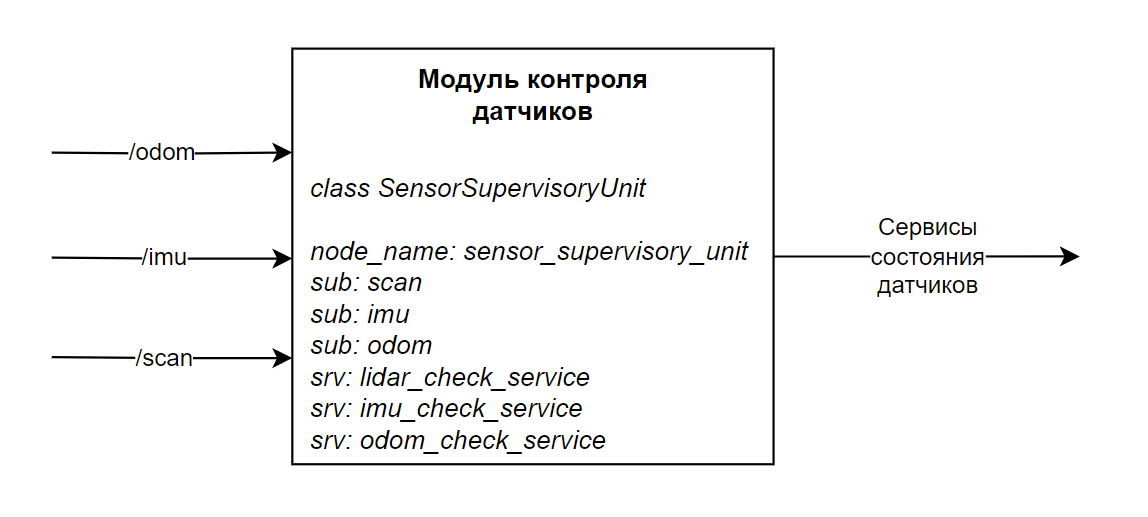
\includegraphics[width=0.6\textwidth]{images/chap_3/sensor_supervisory_unit.png}
    \caption{Модуль контроля датчиков}
    \label{fig:sensor_supervisory_unit}
\end{figure}

\subsection{Модуль навигационных сервисов}

Данный модуль предоставляет сервисы, которые необходимы для проверки системы при навигации робота. 

\begin{figure}[h]
    \centering
    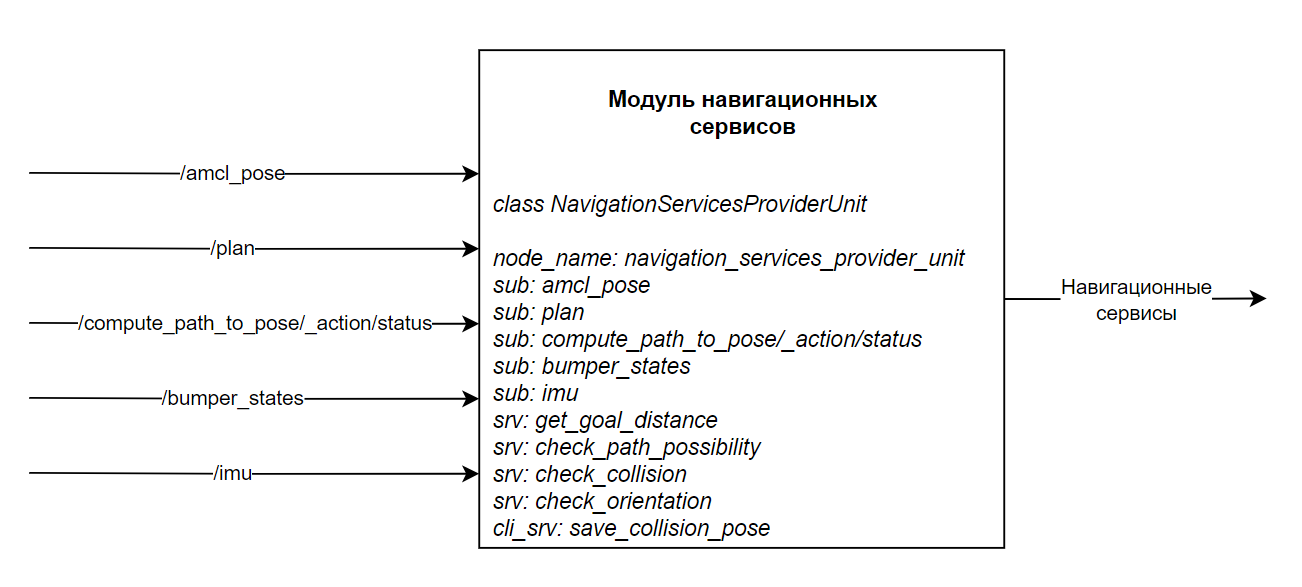
\includegraphics[width=0.75\textwidth]{images/chap_3/navigation_services_unit.png}
    \caption{Модуль навигационных сервисов}
    \label{fig:navigation_services_unit}
\end{figure}

\subsection{Модуль хранения данных}

Модуль хранения данных реализует функционал сбора данных от всех компонентов системы и предоставления их основному поведенческому дереву через соответствующие сервисы. Этот модуль подписывается на все потоки данных датчиков и сохраняет сообщения в очереди. Это означает, что самые последние данные помещаются в массив, а если массив превышает заданную длину, самые старые данные из него удаляются. Таким образом, вычислительная и сетевая нагрузки значительно снижаются. \\
Типы и количество хранимых данных указаны в Таблице \ref*{tab:data_storage}.

\begin{figure}[h]
    \centering
    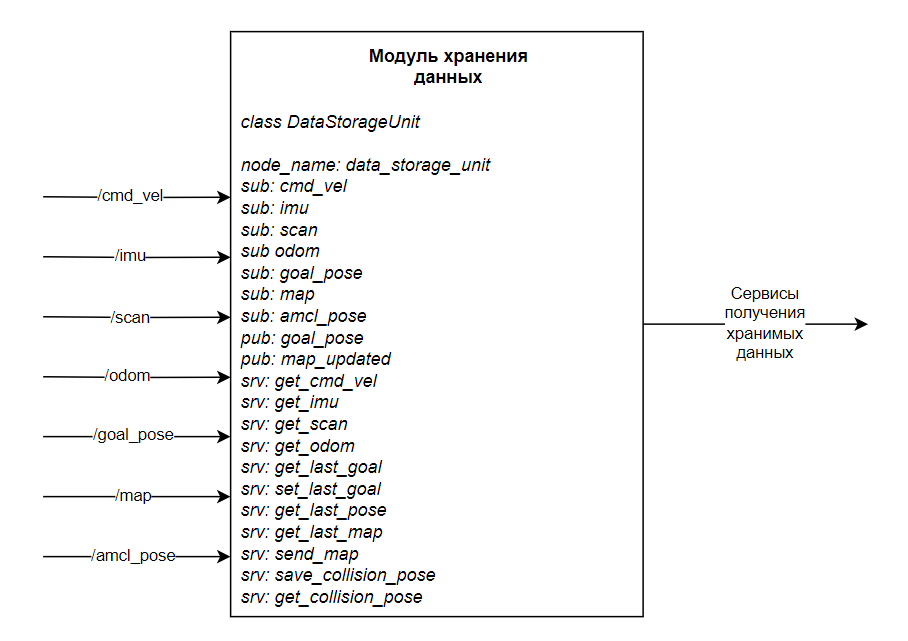
\includegraphics[width=0.75\textwidth]{images/chap_3/data_storage_unit.png}
    \caption{Модуль хранения данных}
    \label{fig:data_storage_unit}
\end{figure}

\begin{table}[]
    \centering
    \begin{tabular}{|c|c|c|}
    \hline
    \textbf{Имя} & \textbf{Тип данных} & \textbf{Объем данных} \\
    \hline
    LIDAR & sensor\_msgs/msg/Laserscan & 3 секунды \\
    \hline
    IMU & sensor\_msgs/msg/Imu & 3 секунды \\
    \hline
    Одометрия & nav\_msgs/Odometry & 3 секунды \\
    \hline
    Положение робота & geometry\_msgs/Pose & 2 секунды \\
    \hline
    Положение при столкновении & geometry\_msgs/Pose & Только последнее \\
    \hline
    Карта занятости & nav\_msgs/OccupancyGrid & Только последняя \\
    \hline
    Сигналы управления & geometry\_msgs/Twist & 3 секунды \\
    \hline
    \end{tabular}
    \caption{Типы и объем данных для хранения}
    \label{tab:data_storage}
\end{table}

\subsection{Модуль переключения управления}

Данный модуль анализирует сообщения от системы Nav2 и основного поведенческого дерева. Сообщения с основного поведенческого дерева имеют больший приоритет, соответственно если данный модуль обнаруживает сообщения в теме \textit{cmd\_vel\_bt}, то сообщения с темы \textit{cmd\_vel\_nav} не будут пропускаться. \\
Также данный модуль реализует сервисы по полной остановке и изменению скорости робота (уменьшение и увеличение). Эти сервисы вызываются когда система обнаруживает сбой некоторых компонент и, для безопасности, требуется ограничить скорость робота или же совсем его остановить.

\begin{figure}[h]
    \centering
    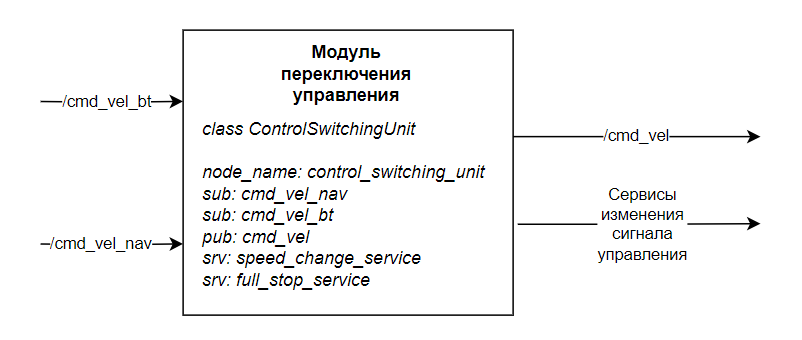
\includegraphics[width=0.6\textwidth]{images/chap_3/control_switching_unit.png}
    \caption{Модуль переключения управления}
    \label{fig:control_switching_unit}
\end{figure}

\subsection{Основное поведенческое дерево}

Данный модуль реализует алгоритм принятия решений всей системы контроля. В основе лежит структура поведенческого дерева, реализованная с помощью библиотеки \textit{BehaviorTree.cpp}.

Структура дерева представляется в виде XML-файла, а поведение отдельных действий объявляется в соответствующих \textit{.hpp} файлах, которые затем регистрируются как узлы деревьев. \\
Ниже представлена высокоуровневая схема дерева.

\begin{figure}[h]
    \centering
    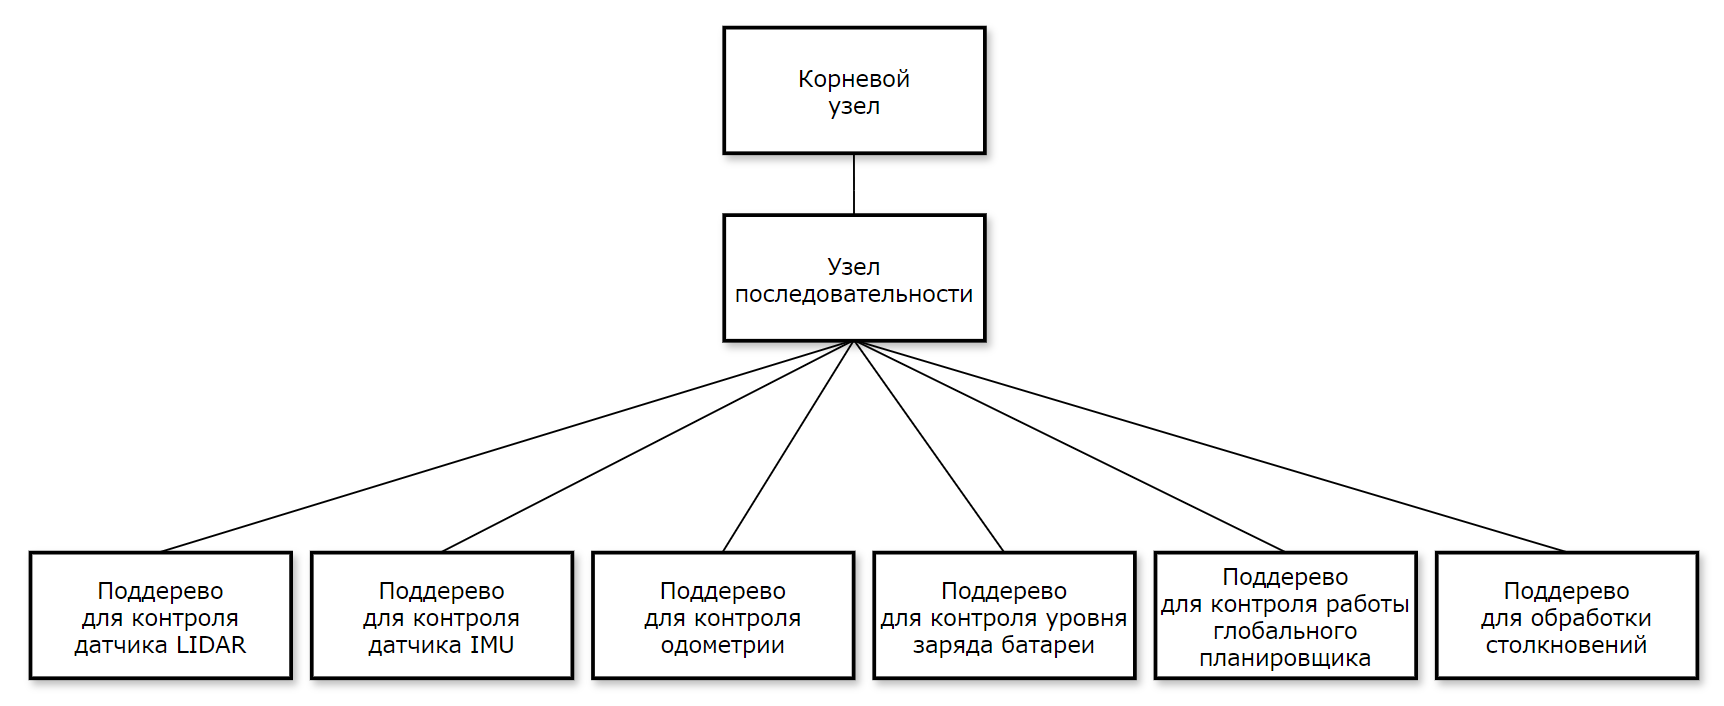
\includegraphics[width=1.0\textwidth]{images/chap_3/subtrees_overview.png}
    \caption{Высокоуровневый граф основного поведенческого дерева}
    \label{fig:subtrees_overview}
\end{figure}

Листья представляют собой поддеревья, которые будут рассмотрены в пунктах далее.
В качестве главного узла управления выбран последовательный узел. \\
Соответственно, все потомки последовательного узла расположены в порядке увеличения сложности функционирования. То есть вначале идут низкоуровневые компоненты, без работы которых функционирование системы невозможно. А справа более высокоуровневые, которые требует выполнения всех компонентов левее от себя.

\subsubsection{Поддеревья для контроля датчиков}

\begin{figure}[h]
    \centering
    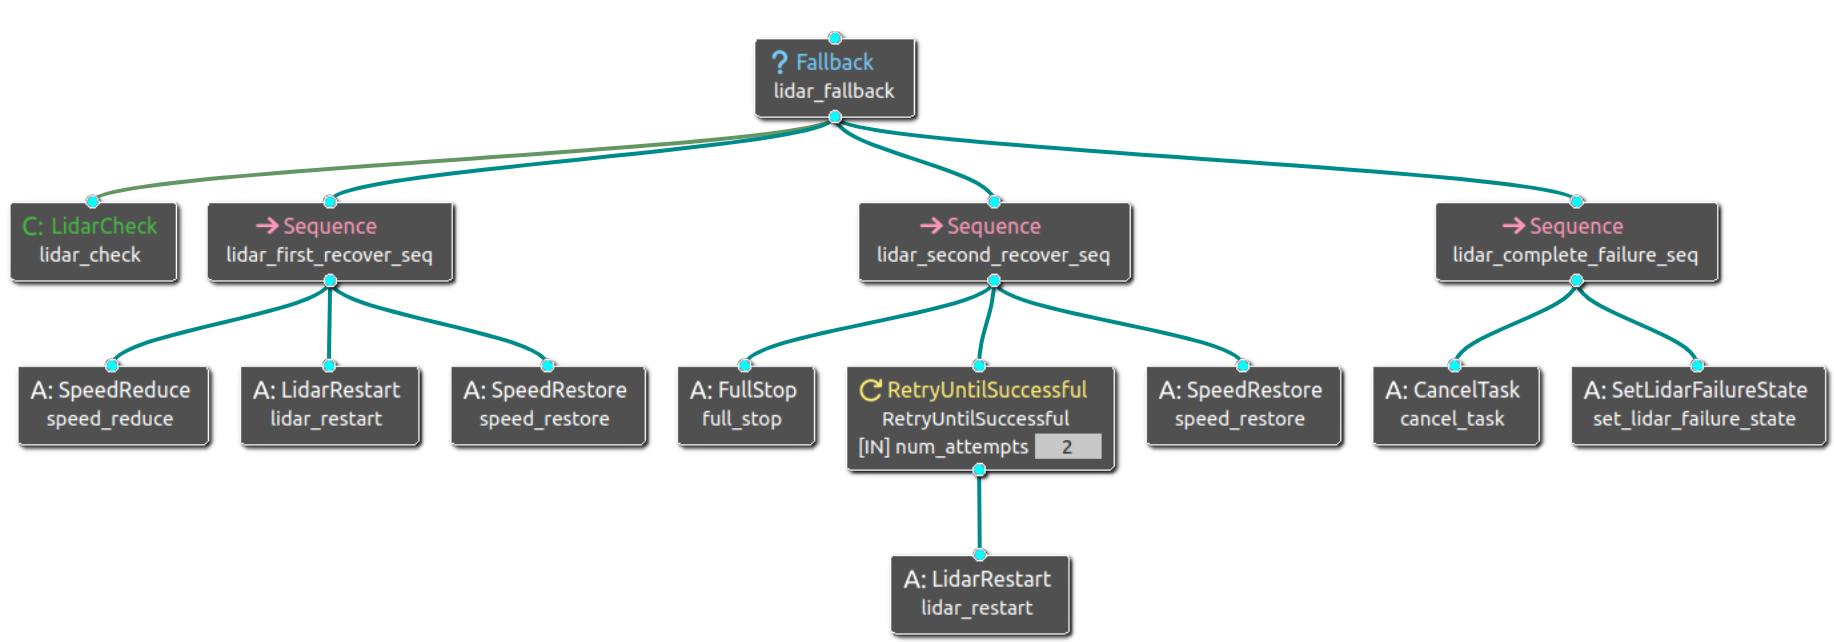
\includegraphics[width=1.0\textwidth]{images/chap_3/sensor_subtree.png}
    \caption{Поддерево для контроля датчика LIDAR}
    \label{fig:sensor_subtree}
\end{figure}

На Рисунке \ref*{fig:sensor_subtree} находится схема поддерева для проверки работоспособности датчика LIDAR (поддеревья для датчиков IMU и проверки одометрии аналогичны).

Модуль основного поведенческого дерева вызывает сервисы проверки датчиков в узлах-условиях (condition nodes), реализованные в модуле контроля датчиков. Если узел условия \textit{collision\_check} (вызывающий сервис проверки) возвращает "Успех", то датчик LIDAR в норме и проход данного поддерева завершается. Иначе, сигнал прохода идет в узел последовательности \textit{collision\_handle\_seq}. \\
Обработка данной ситуации выполняет следующие действия:
\begin{enumerate}
    \item Снижение скорости до минимально допустимой, попытка перезагрузить модуль сенсора и, в случае успешной перезагрузки, восстановление скорости
    \item Если же после первой перезагрузки модуля сенсора, сенсор продолжает не работать, следует полная остановка робота, далее производятся 2 попытки перезагрузки, и в случае если сенсор заработал - восстановление скорости
    \item Если же 2 предыдущие последовательности не смогли возвратить функционирование сенсору - происходит отмена всех целей навигации робота и введение системы в состояние ошибки
\end{enumerate}

Время которое должно пройти с последнего сообщения от датчика для того чтобы модуль контроля датчиков объявил о неисправности датчика равно 1 секунде. По истечению данного времени робот будет недолго продолжать движение к цели. Однако если не удастся восстановить функционирование датчика - робот больше не сможет безопасно функционировать, а значит следует его полная остановка. \\
Такое поведение реализовано для датчиков LIDAR и IMU, а также для системы одометрии. Так как данные компоненты являются критически важными для безопасного функционирования, то в случае любых неисправностей навигация прекращается.

\subsubsection{Поддерево для контроля уровня заряда батареи}

\begin{figure}[h]
    \centering
    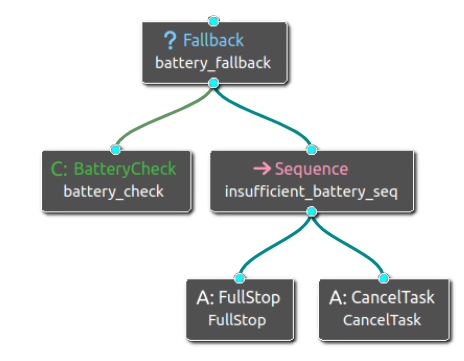
\includegraphics[width=0.4\textwidth]{images/chap_3/battery_subtree.png}
    \caption{Поддерево для контроля уровня заряда батареи}
    \label{fig:battery_subtree}
\end{figure}

Данное поддерево реализует проверку заряда батареи для успешного выполнения задачи навигации. Проверка основывается на значениях текущего заряда батареи, среднего потребление батареи и длины пути до цели. \\
Задача навигации будет отменена, если будет установлено, что уровня заряда не хватит до достижения цели.

Для реализации данного поведения был создан ROS пакет для симуляции компонента батареи у мобильного робота (модуль симуляции батареи). У данного модуля есть сервис через который модуль основного поведенческого дерева может получить уровень заряда и, проведя операции, определить достаточен ли уровень.

\subsubsection{Поддерево для контроля работы глобального планировщика}

\begin{figure}[h]
    \centering
    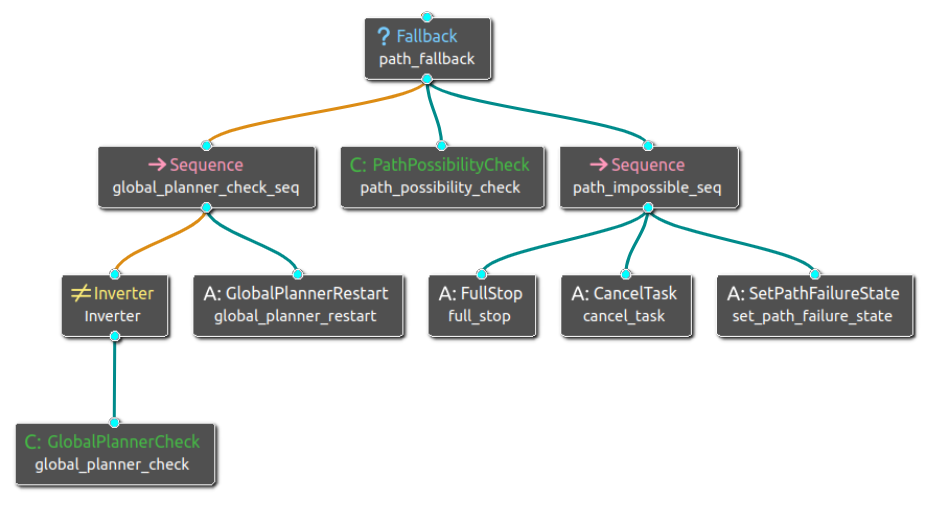
\includegraphics[width=0.8\textwidth]{images/chap_3/global_planner_subtree.png}
    \caption{Поддерево для контроля работы глобального планировщика}
    \label{fig:global_planner_subtree}
\end{figure}

Данное поддерево реализует поведение для проверки работоспособности планировщика траектории. Так как узел \textit{GlobalPlanner} модуля Nav2 является узлом типа \textit{LifecycleNode}, то информацию о его состоянии можно получить с помощью вызова соответствующего сервиса. 

В основе \textit{LifecycleNode} лежит следующий конечный автомат состояний:

\begin{figure}[h]
    \centering
    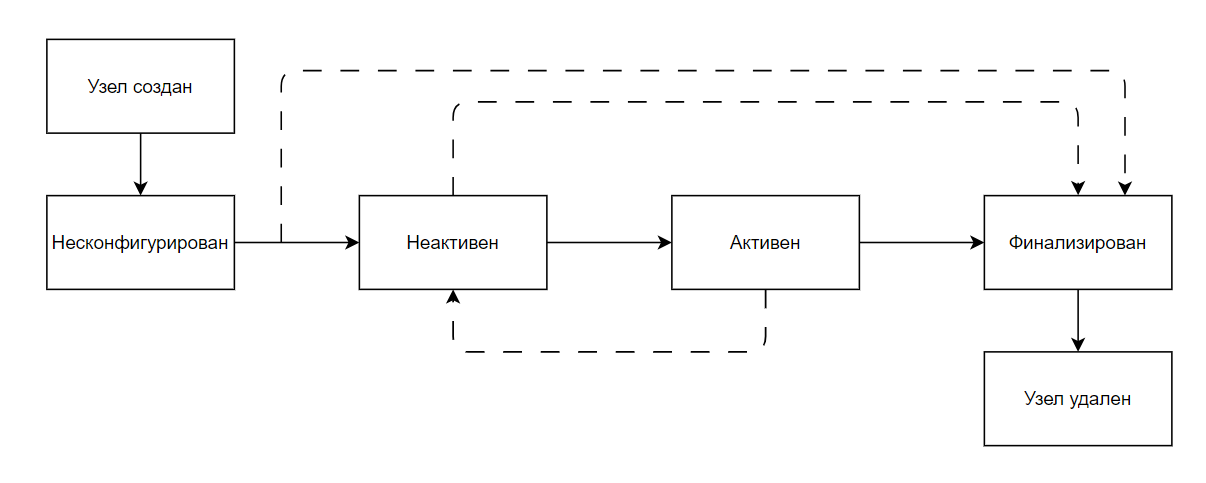
\includegraphics[width=0.7\textwidth]{images/chap_3/lifecycling.png}
    \caption{Конечный автомат узла жизненного цикла}
    \label{fig:lifecycling}
\end{figure}

Следовательно обращаясь непосредственно к соответствующему сервису узла глобального планировщика мы получаем информацию в каком состоянии он находится. 

Также при проходе данного поддерева происходит проверка на достижимость поставленной точки на карте (цели навигации) с помощью просмотра состояния вызванного действия (там тоже используется конечный автомат) \textit{NavigateToPose} узла \textit{bt\_navigator} модуля Nav2.

\begin{figure}[h]
    \centering
    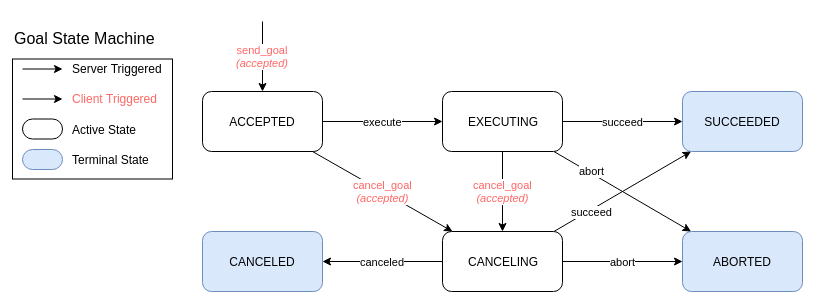
\includegraphics[width=0.7\textwidth]{images/chap_3/action_fsm.png}
    \caption{Конечный автомат для действия в ROS2}
    \label{fig:action_fsm}
\end{figure}

Таким образом реализуется поведение, которое проверяет работу планировщика пути и может устранить автономно некоторые неполадки или же уведомить об ошибке.

\subsubsection{Поддерево для обработки столкновений}

\begin{figure}[h]
    \centering
    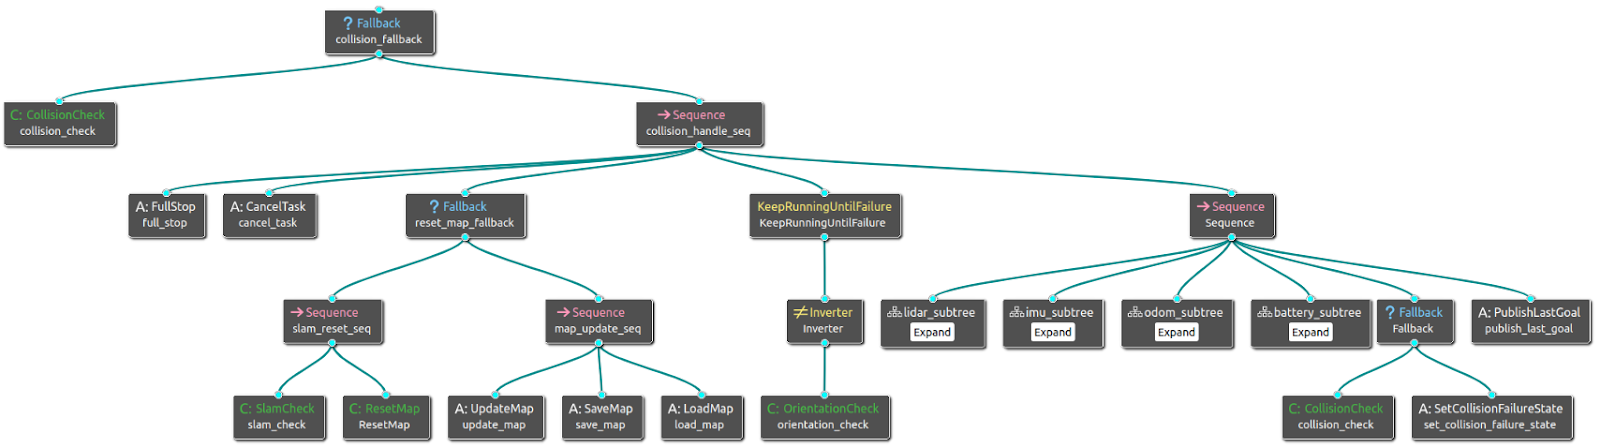
\includegraphics[width=1.0\textwidth]{images/chap_3/collision_subtree.png}
    \caption{Поддерево для обработки столкновений}
    \label{fig:collision_subtree}
\end{figure}

Данное поддерево реализует поведение при столкновениях робота с объектами. \\
Необходимо обнаруживать столкновения, обновлять карту местности (добавление препятствия) и перестраивать путь до цели с учетом новой карты.

Для обнаружения препятствий к передней части робота был добавлен датчик столкновений, который способен детектировать столкновения перед собой и публиковать информацию в тему \textit{/bumper\_states}. Далее на это подписывается модуль навигационных сервисов и предоставляет сервис через который основное поведенческое дерево узнает был ли робот в состоянии столкновения с объектом в последние 0.5 секунд или нет. При столкновении модуль навигационных сервисов запоминает положение и ориентацию робота в последний момент перед столкновением для того, чтобы далее передать эту информацию для добавления препятствия на карту местности. 

После того как было обнаружено столкновение, происходит полная остановка робота и отмена всех целей навигации. Затем проверятеся функционирует ли робот в режиме SLAM или же карта местности была заранее загружена в память с помощью Map server. В зависимости от этого происходит либо полный сброс карты, либо же обновление карты.
Действие \textit{UpdateMap} соответвенно добавляет препятствие в виде квадрата 0.25х0.25 м перед роботом.

Далее робот переводится в режим ожидания до тех пор, пока не будет восстановлена его ориентация в пространстве. \\ 
Проверка ориентации в пространсве происходит через анализ данных, поступающих с инерциального измерительного блока. Датчик IMU посылает сигналы типа данных \textit{sensor\_msgs/Imu}. В объектах этого класса присутствуют следующие поля:
\begin{itemize}
    \item \textit{Header header}
    \item \textit{geometry\_msgs/Quaternion orientation}
    \item \textit{float64[9] orientation\_covariance}
    \item \textit{geometry\_msgs/Vector3 angular\_velocity}
    \item \textit{float64[9] angular\_velocity\_covariance}
    \item \textit{geometry\_msgs/Vector3 linear\_acceleration}
    \item \textit{float64[9] linear\_acceleration\_covariance}
\end{itemize}

Для проверки ориентации мы используем поле \textit{orientation}, записанное в виде кватерниона. Преобразуем его в матрицу поворота с помощью библиотеки \textit{tf2}, далее из этой матрицы поворота извлекаем углы крена, тангажа и рыскания и проверяем чтобы они лежали в диапазоне от -6 до 6 градусов. Данную проверку осуществляет модуль навигационных сервисов при вызове соответствующего сервера.

После восстановления ориентации происходит проверка всех важных компонент системы (LIDAR, IMU, одометрия, батарея) и если хотя бы один из модулей работает некорректно, робот переходит в состояние неисправности. Такой случай означает то, что в результате столкновения был поврежден какой-то критически важный компонент. \\
Если же все критически важные компоненты работают исправно, то происходит еще одна проверка на состояние столкновения. В данной работе для гарантий безопасности робот не будет продолжать движение, если датчик столкновения фиксирует контакт с другим объектом. Движение может продолжиться только в случае отсутствия контакта. \\ 
Соответственно, при отсутствии контакта, восстанавливается прошлая цель навигации и планировщик пути стоит новую траекторию с учетом отмеченного на карте объекта столкновения.

\subsection{Дополнительные модули}

\subsubsection{Модуль симуляции батареи}

\begin{figure}[h]
    \centering
    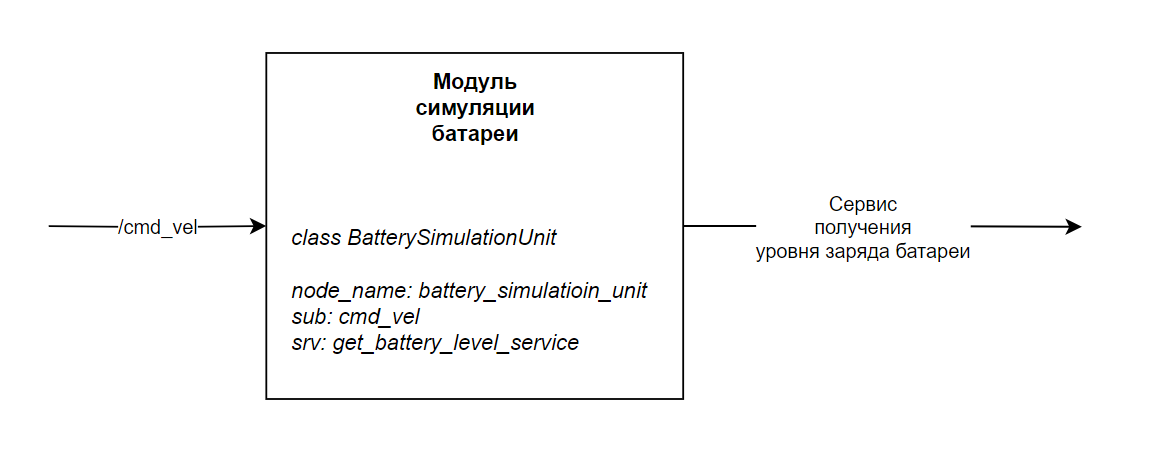
\includegraphics[width=0.7\textwidth]{images/chap_3/battery_sim_unit.png}
    \caption{Модуль симуляции батареи}
    \label{fig:battery_sim_unit}
\end{figure}

Для тестирования поведения системы при недостаточном уровне заряда был реализован модуль симуляции батареи робота. \\
Модуль принимает информацию о текущей скорости робота и в соответствии с заданными параметрами рассчитывает уровень заряда. \\
Параметры:
\begin{itemize}
    \item расход батареи при простое;
    \item коэффициент расхода батареи при движении - линейно зависит от скорости робота;
    \item стартовый уровень заряда - в процентах.
\end{itemize}

В модуле также реализован интерфейс по которому другие модули системы могут узнать текущий уровень заряда \textit{get\_battery\_level\_service}.

\subsubsection{Модуль симуляции неисправностей}

\begin{figure}[h]
    \centering
    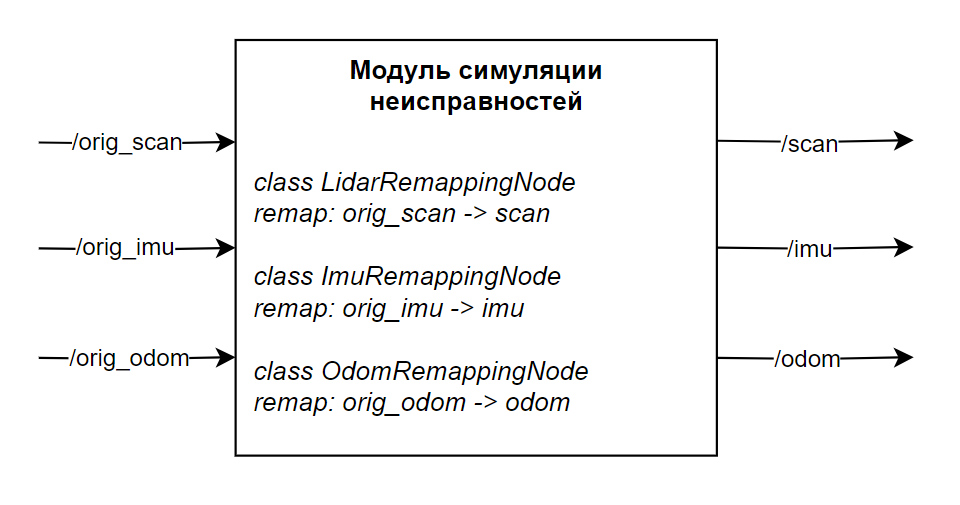
\includegraphics[width=0.7\textwidth]{images/chap_3/failure_sim_unit.png}
    \caption{Модуль симуляции неисправностей}
    \label{fig:failure_sim_unit}
\end{figure}

Для тестирования поведения системы при неисправностях датчиков LIDAR и IMU, а также одометрии был реализован модуль симуляции неисправностей.\\
Все данные с этих компонент проходят через этот модуль, для того чтобы имелась возможность приостановить потоки данных. Это реализовано в виде перенаправления тем (topic remappings). \\
В итоге, приостановка одного из узлов данного модуля симулирует неисправность соответствующей компоненты.

\subsubsection{Модуль пользовательских интерфейсов системы}

Так как основной способ передачи данных между модулями являются сервисы, то для их корректной работы потребовалось создать соответствующие им типы данных - интерфейсы.

\begin{table}[h]
    \centering
    \resizebox{\textwidth}{!}{%
    \begin{tabular}{|c|c|c|}
        \hline
        \textbf{Имя сервиса} & \textbf{Тип запроса} & \textbf{Тип ответа} \\
        \hline
        GetBatteryLevel.srv & std\_msgs/Empty empty\_request & \begin{tabular}{@{}l@{}@{}}float64 battery\_level \\ float64 idle\_consumption \\ float64 drive\_consumption\end{tabular} \\
        \hline
        GetGoal.srv & std\_msgs/Empty empty\_request & geometry\_msgs/Pose goal\_pose \\
        \hline 
        GetGoalDistance.srv & std\_msgs/Empty empty\_request & float64 goal\_distance \\
        \hline 
        GetLastMap.srv & std\_msgs/Empty empty\_request & nav\_msgs/OccupancyGrid map \\
        \hline 
        GetPose.srv & std\_msgs/Empty empty\_request & geometry\_msgs/Pose pose \\
        \hline 
        PubResCmdVel.srv & geometry\_msgs/Twist cmd\_vel & bool success \\
        \hline 
        SendMap.srv & nav\_msgs/OccupancyGrid map & std\_msgs/Empty empty\_response \\
        \hline
    \end{tabular}}
    \caption{Описание реализованных интерфейсов для системы контроля}
    \label{tab:my_label}
\end{table}

\section{Система учета динамических объектов}

\subsection{Принципы обхода препятствий в Nav2}

В системе Nav2 планирование траектории движения разделено на 2 уровня:
\begin{enumerate}
    \item Сервер планирования (глобальный планировщик) - строит полный оптимальный путь от начального положения робота до цели навигации. Он принимает на вход статическую карту местности (либо заранее созданную, либо динамически обновляемую с помощью SLAM), а также может принимать некоторые другие слои карты (слой препятствий, слой инфляции, слой вокселов). Все слои накладываются друг на друга и на выходе дают объект класса \textit{2DCostmap}. В итоге получается карта стоимости, представляющая собой сетчатую карту, в каждой ячейке которой записана стоимость нахождения робота в ней. Сервер планирования работает с этим результирующим объектом (глобальная карта стоимости).
    \item Сервер управления (локальный планировщик) - вычисляет сигнал управления для слежения за траекторией построенной глобальным планироващиком. По аналогии с сервером планирования, у сервера управления также имеется в наличии локальная карта стоимости. Однако она имеет меньший размер, иную конфигурацию слоев и большую частоту обновления.
\end{enumerate}

Соответственно отсюда мы видим, что обработка новых, заранее не отмеченных на статической карте объектов (в том числе динамических) происходит на уровне локального планировщика. Следовательно, если мы хотим как-то учитывать динамические препятствия, то необходимо модифицировать работу локального планировщика.

Работа основных серверов системы Nav2 (сервер навигации, сервер планирования, сервер управления, сервер восстановления) основывается на использовании плагинов: как уже существующих и предоставляемых разработчиками Nav2, так и пользовательских (для введения новых особенностей).

Для вычисления траектории сервер планирования по умолчанию использует плагин \textit{NavfnPlanner}. Данный алгоритм планирования основан на применении алгоритма Дейкстры. Модифицировать работу глобального планировщика нет нужды, так как обработка динамических объектов должна происходить на уровне сервера управления.

Сервер управления, в свою очередь, может использовать для вычисления траектории в динамическом окружении два плагина (предоставляемых Nav2):
\begin{enumerate}
    \item DWB контроллер (\textit{nav2\_dwb\_controller} \cite{nav2-dwb})
    \item TEB контроллер (\textit{teb\_local\_planner} \cite{teb-planner})
\end{enumerate}

DWB контроллер - это плагин, реализующий подход динамического окна. Он учитывает все скорости, которые робот может достичь за промежуток времени между двумя последовательными сигналами управления. Скорости, которые могут привести к столкновениям, исключаются. Среди оставшихся скоростей выбирается наиболее перспективные сигналы управления с помощью функции затрат, представленной в виде карты стоимости (локальной), которая определяет стоимость прохождения через каждую ячейку карты \cite{dwa}.

Контроллер TEB - это реализация подхода эластичной ленты. Он использует полный, свободный от препятствий путь от начальной точки до точки цели навигации. Этот путь разбивается на участки, которые затем переставляются под воздействием вновь обнаруженных препятствий с помощью модели сил. Сила, действующая между участками, удерживает их вместе, а сила отталкивания толкает путь в сторону от препятствий. TEB расширяет данный метод, добавляя дополнительную информацию о времени участкам пути. Используя эту информацию, функция стоимости может учитывать как время движения, так и расстояние до препятствий \cite{teb-info}.

\subsection{Описание работы предлагаемой системы}

Контроллер DWB, используемый по умолчанию сервером управления для построения траектории на основе локального представления (\textit{local\_costmap}), обращается с новыми (заранее не отмеченными препятствиями на статической карте) статическими и динамическими объектами одинаково. \\
В простейшем случае - данные с 2D LIDAR обрабатываются и отмечаются в слое \textit{obstacle\_layer}, далее накладывается \textit{inflation\_layer} для добавления “запаса безопасности” - экспоненциально убывающая функция стоимости от расстояния соседних клеток до препятствия. \\ 
В процессе движения динамического препятствия карта обновляется в соответствии с указанными параметрами. \\
В таком случае локальный планировщик не имеет информации о скорости и направлении движения объекта, а значит он не может спрогнозировать ситуацию, когда динамический объект будет пересекать построенную траекторию движения робота. При пересечении объектом построенной траектории движения планировщиком будут вызываться попытки перестроить траекторию, однако из-за отсутствия информации о величине и направлении скорости препятствия, будут происходить случаи, когда объект будет пересекать минимально допустимое расстояние до робота. Это вызовет поведение восстановления \textit{wait} сервером восстановления и мобильный робот будет ждать до тех пор, пока динамический объект не покинет зону близости.

Соответственно для уменьшения таких ситуаций было предложено следующее решение, основанное на работе \cite{albers2019online}. Предлагаемая система учета динамических объектов состоит из следующих модулей:
\begin{itemize}
    \item модуль обнаружения динамических объектов;
    \item модуль слежения за обнаруженными объектами и оценки их скоростей;
    \item модуль отображения информации об объектах на карте стоимости.
\end{itemize}

Итого, данная система реализует учет динамических объектов в среде с помощью их отслеживания и представления информации о скорости движения в качестве плагина для добавления слоя в локальную карту стоимости.

\subsection{Архитектура системы}

\begin{figure}[h]
    \centering
    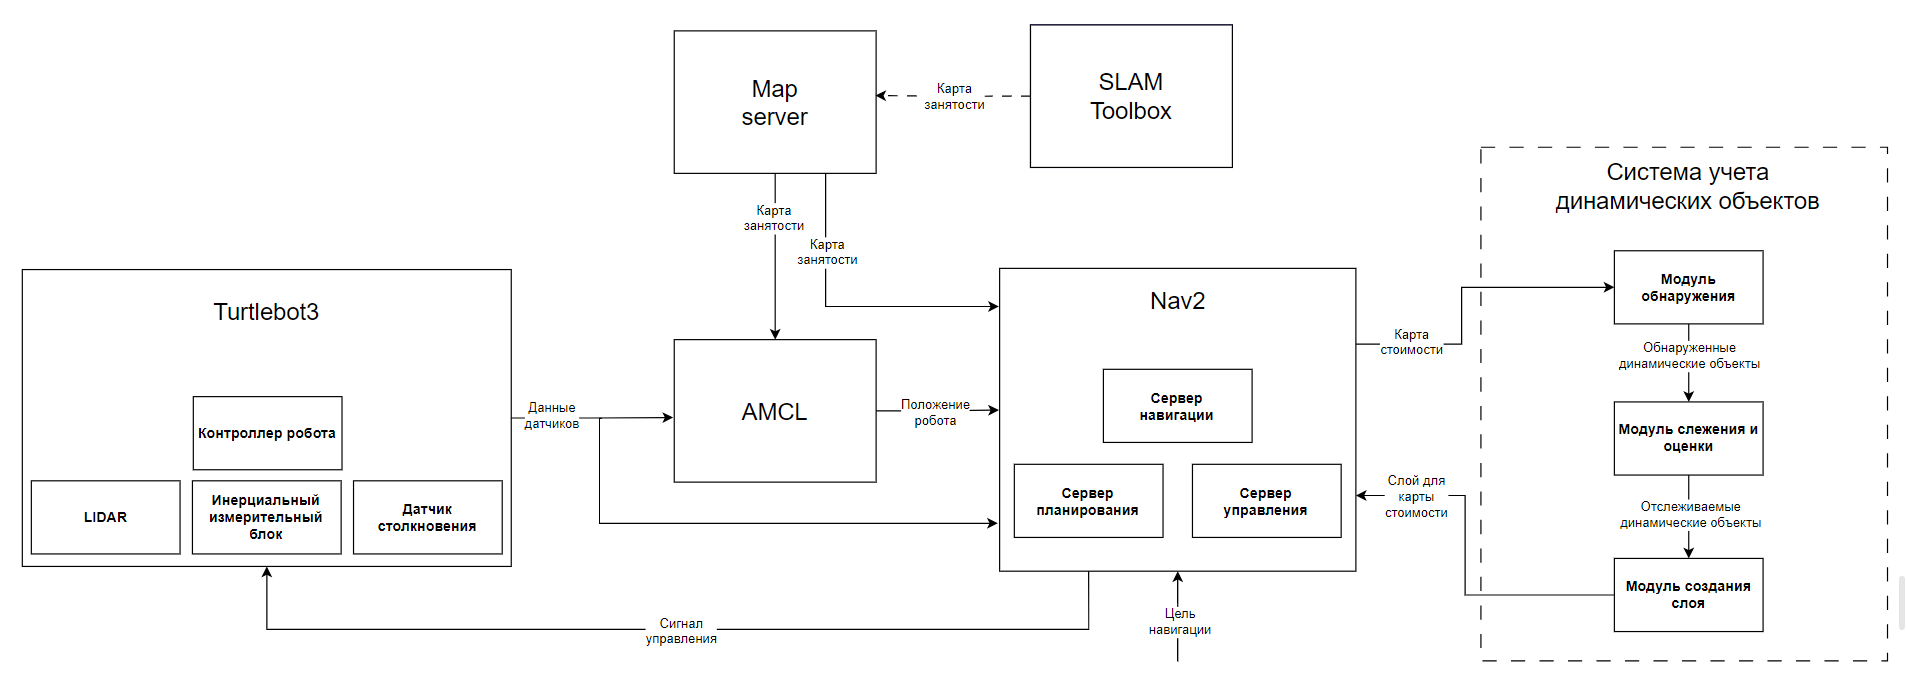
\includegraphics[width=1.0\textwidth]{images/chap_3/dyn_obs_av_sys_arch.png}
    \caption{Архитектура системы учета динамических объектов}
    \label{fig:dyn_obs_av_sys_arch}
\end{figure}

На Рисунке \ref*{fig:dyn_obs_av_sys_arch} представлена архитектура системы учета динамических препятствий. Она состоит из трех модулей: модуль обнаружения динамических препятствий, модуль слежения за перпятствиями и оценки их скорости и модуль добавления динамических объектов на новый слой для локальной карты стоимости.

\subsection{Модуль обнаружения}

\begin{figure}[h]
    \centering
    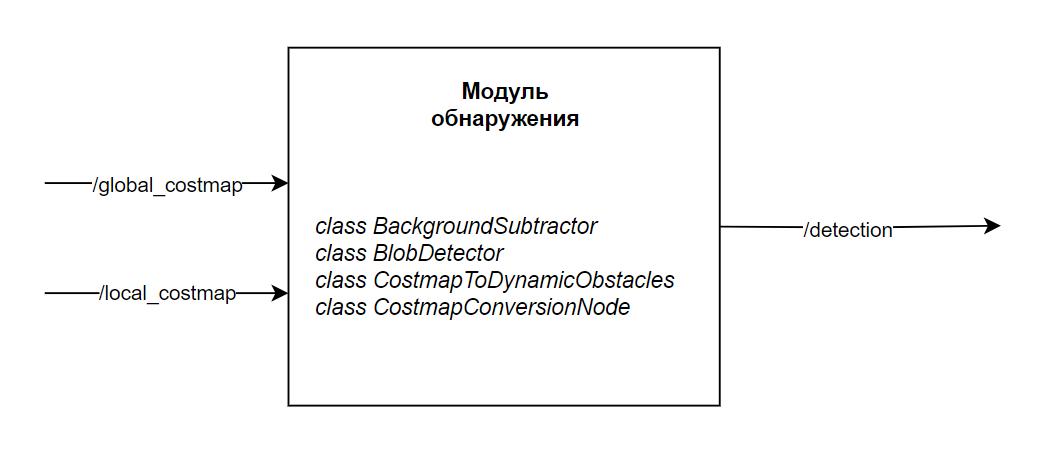
\includegraphics[width=0.7\textwidth]{images/chap_3/costmap_conversion.png}
    \caption{Модуль обнаружения динамических объектов}
    \label{fig:costmap_conversion}
\end{figure}

Объект класса \textit{CostmapConversionNode} является главным и управляет ходом процесса выделения динамических объектов из карты стоимости. \\ 
При инициализации происходит создание подписчика (subscriber) на темы \textit{/global\_costmap} и \textit{/local\_costmap} и издателя (publisher) темы \textit{/detection}. В тему \textit{/detection} с определенным интервалом времени будет передаваться массив \textit{ObstacleArray.msg} из детектированных динамических объектов (имеющих пользовательский тип данных \textit{Obstacle.msg}). \\
Процесс обнаружения динамических объектов также будет выполняться с частотой публикации данных в тему \textit{/detection}.

Функционал преобразования карты местности в массив динамических объектов определен в классе \textit{CostmapToDynamicObstacles}. Этот процесс состоит из следующих шагов:
\begin{enumerate}
    \item \textit{CostmapToDynamicObstacle::setCostmap2D()} - преобразование карты стоимости из типа \textit{nav2\_costmap\_2d::Costmap2D} в тип данных \textit{cv::Mat}, для того чтобы можно было применять методы библиотеки OpenCV
    \item \textit{BackgroundSubtractor::apply()} - применение фильтров, в результате динамические объекты будут отражены в бинарной матрице \textit{fg\_mask} 
    \item \textit{BlobDetector::detect()} - применение кластеризации и вычисление центров динамических объектов. Реализованый класс \textit{BlobDetector} наследован от класса \textit{SimpleBlobDetector} библиотеки OpenCV \cite{simple-blob-opencv}
    \item Запись всех обнаруженных объектов в \textit{ObstacleArray.msg}
\end{enumerate}

На Рисунке \ref*{fig:example_costamp_converter} представлен результаты работы данного модуля в ситуации с одним динамическим объектом, движущимся по короткой стороне карты.

\begin{figure}[H]
    \centering
    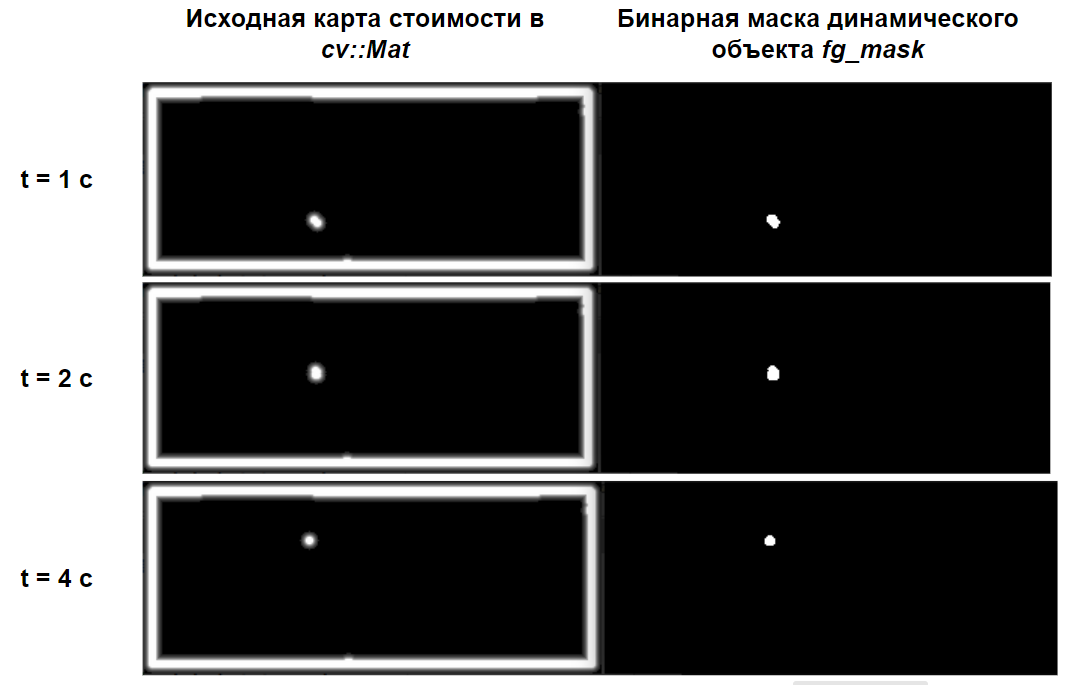
\includegraphics[width=0.8\textwidth]{images/chap_3/example_costamp_converter.png}
    \caption{Результат работы модуля обнаружения динамических объектов}
    \label{fig:example_costamp_converter}
\end{figure}

Как видно, выделение динамических объектов было проведено успешно. Удалось отфильтровать статические объекты и выделить только динамические. 

\subsection{Модуль слежения и оценки}

\begin{figure}[h]
    \centering
    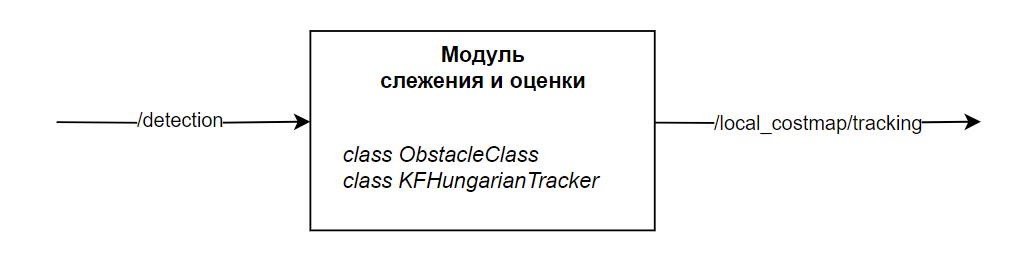
\includegraphics[width=0.7\textwidth]{images/chap_3/tracking_est.png}
    \caption{Модуль слежения и оценки динамических объектов}
    \label{fig:tracking_est}
\end{figure}

Классс \textit{ObstacleClass} представляет собой один динамический объект, его поля хранят необходимую о динамическом объекте информацию:
\begin{itemize}
    \item положение;
    \item скорость;
    \item фильтр Калмана типа \textit{cv2.KalmanFiler};
    \item количество фреймов (снимков), в которых данный объект отсутствовал (при достижении порогового значения - объект удаляется).
\end{itemize}

Отметим, что \textit{cv2.KalmanFiler} - это класс библиотеки OpenCV \cite{kalman-filter-opencv}, который реализует шаги предсказания и обновления фильтра Калмана через методы \textit{cv2.KalmanFilter.predict()} и \textit{cv2.KalmanFilter.update()}. При создании объекта этого класса матрицы $H, F, R, P, Q$ инициализируются, как указано в подразделе 1.3.2.

Класс \textit{KFHungarianTracker} реализует процесс слежения за динамическими объектами. Он подписывается на тему \textit{/detection} (с которого поступают данные об обнаруженных динамических объектах), и публикует данные об отслеживаемых объектах в тему \textit{/local\_costmap/tracking}. \\
При каждом новом поступлении данных выполняются следующие действия:
\begin{enumerate}
    \item Вычисляется промежуток времени между сообщениями для того чтобы передать его в метод \textit{predict()} класса \textit{ObstacleClass}, тем самым предсказав положение и скорость детектированных объектов
    \item Далее решается задача сопоставления объектов (assignment problem) с помощью венгерского алгоритма. Для этого используется функция \textit{linear\_sum\_assignment()} библиотеки SciPy \cite{lin-sum-ass-scipy}
    \item Имея информацию о парах объектов (объект в момент $t$ и тот же объект в момент $t+1$), мы обновляем фильтр Калмана для сооветствующих объектов (метод \textit{correct()} класса \textit{ObstacleClass})
    \item В конце массив отслеживаемых объектов публикуется в тему \textit{/local\_costmap/tracking}
\end{enumerate}

На Рисунке \ref*{fig:tracking-example} представлен пример выделения двух динамических объектов и оценки их скорости.

\begin{figure}[H]
    \centering
    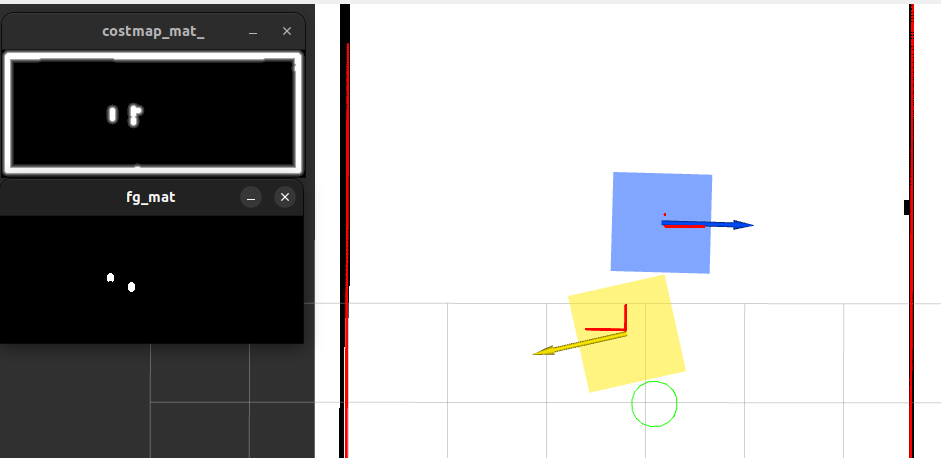
\includegraphics[width=0.9\textwidth]{images/chap_3/tracking-example.png}
    \caption{Пример работы модуля слежения и оценки динамических объектов}
    \label{fig:tracking-example}
\end{figure}

Два динамических объекта были обнаружены и производится слежение за ними, а также оценка из скоростей. Динамические объекты сегментированы в виде прямогульников, а также показана оценка величины и направления скорости (в виде векторов, идущих из центров прямоугольников).

\subsection{Модуль добавления слоя}

\begin{figure}[H]
    \centering
    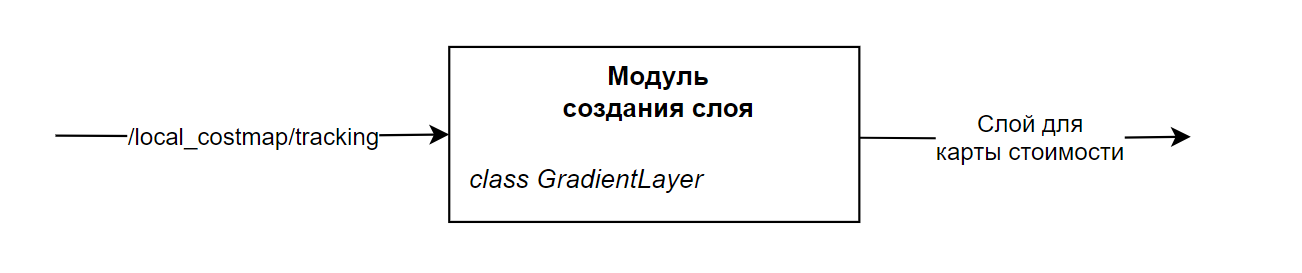
\includegraphics[width=0.7\textwidth]{images/chap_3/layes_creation.png}
    \caption{Модуль добавления слоя}
    \label{fig:layes_creation}
\end{figure}

Данный модуль создавался по шаблону предложенному разработчиками Nav2 для создания пользовательского плагина для реализации слоя для карты стоимости \cite{layer-plugin-nav2}.

Основной класс \textit{GradientLayer} вычисляет и добавляет область стоимости около каждого динамического объекта через метод \textit{updateCosts()}, который выполняет следующие действия: 
\begin{enumerate}
    \item Получает текущие отслеживаемые динамические объекты из темы \textit{/local\_costmap/tracking}
    \item Меняет систему координат относительно которой записаны динамические объекты (\textit{map -> odom}). Так как \textit{local\_costmap} использует систему координат \textit{/odom}, а мы как раз хотим применить наш слой к \textit{local\_costmap}
    \item Добавление к каждому динамическому объекту области стоимости в соответствующей формы (описано в подразделе 1.3.3), в зависимости от направления и величины скорости объекта. Данный функционал реализован в функции \textit{markDynamicObstacle()}
\end{enumerate}

На Рисунке \ref*{fig:layer-example} представлена локальная карта местности с применением данного \textit{GradientLayer}:

\begin{figure}[H]
    \centering
    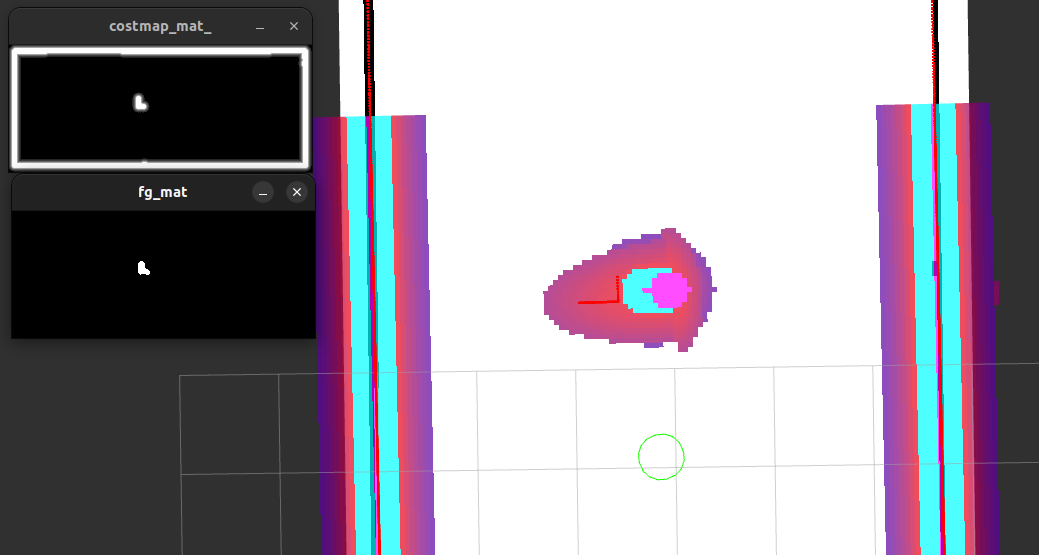
\includegraphics[width=0.9\textwidth]{images/chap_3/layer-example.png}
    \caption{Пример работы модуля добавления слоя}
    \label{fig:layer-example}
\end{figure}

Опишем работу данного модуля на основе приведенного примера. Динамический объект совершает движение налево. Система динамического учета обнаруживает, отслеживает и оценивает величину и направление скорости динамического объекта. В соответствии с этим на локальную карту местности добавилась гауссовская область затрат, распределенная таким образом, что затраты по направлению движения больше, чем за объектом. Таким образом локальный планировщик будет учитывать информацию о скорости динамического препятствия.

\subsection{Модуль пользовательских интерфейсов системы}

Для представления динамических объектов был создан класс \textit{DynamicObstacle}. Для передачи объектов между модулями необходимо было реализовать пользовательский интерфейс. \\
Он реализован в качестве двух типов сообщений:
\begin{enumerate}
    \item \textit{Obstacle.msg}
\begin{figure}[H]
    \centering
    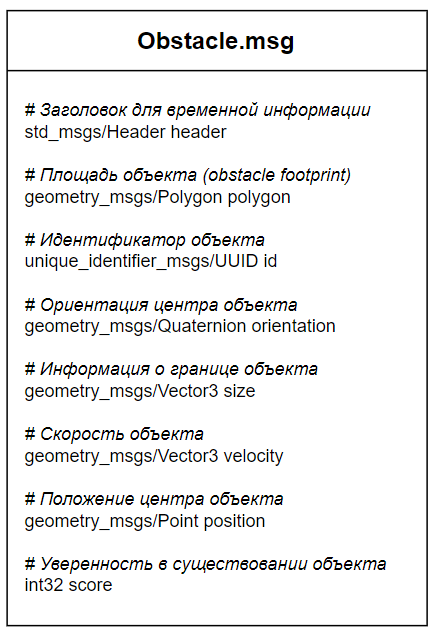
\includegraphics[width=0.4\textwidth]{images/chap_3/obstaclemsg.png}
    \caption{\textit{Obstacle.msg}}
    \label{fig:obstaclemsg}
\end{figure}
    \item \textit{ObstacleArray.msg}
\begin{figure}[H]
    \centering
    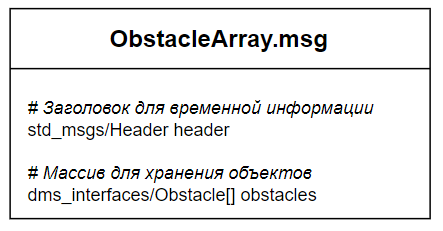
\includegraphics[width=0.4\textwidth]{images/chap_3/obstaclearraymsg.png}
    \caption{\textit{ObstacleArray.msg}}
    \label{fig:obstaclearraymsg}
\end{figure}
\end{enumerate}

Оба типа сообщений находятся в общем пакете \textit{dms\_interfaces}, вместе с интерфейсами для системы контроля.

\section{Общая архитектура системы принятия решений}

Итоговая архитектура разработанной системы:

\begin{figure}[H]
    \centering
    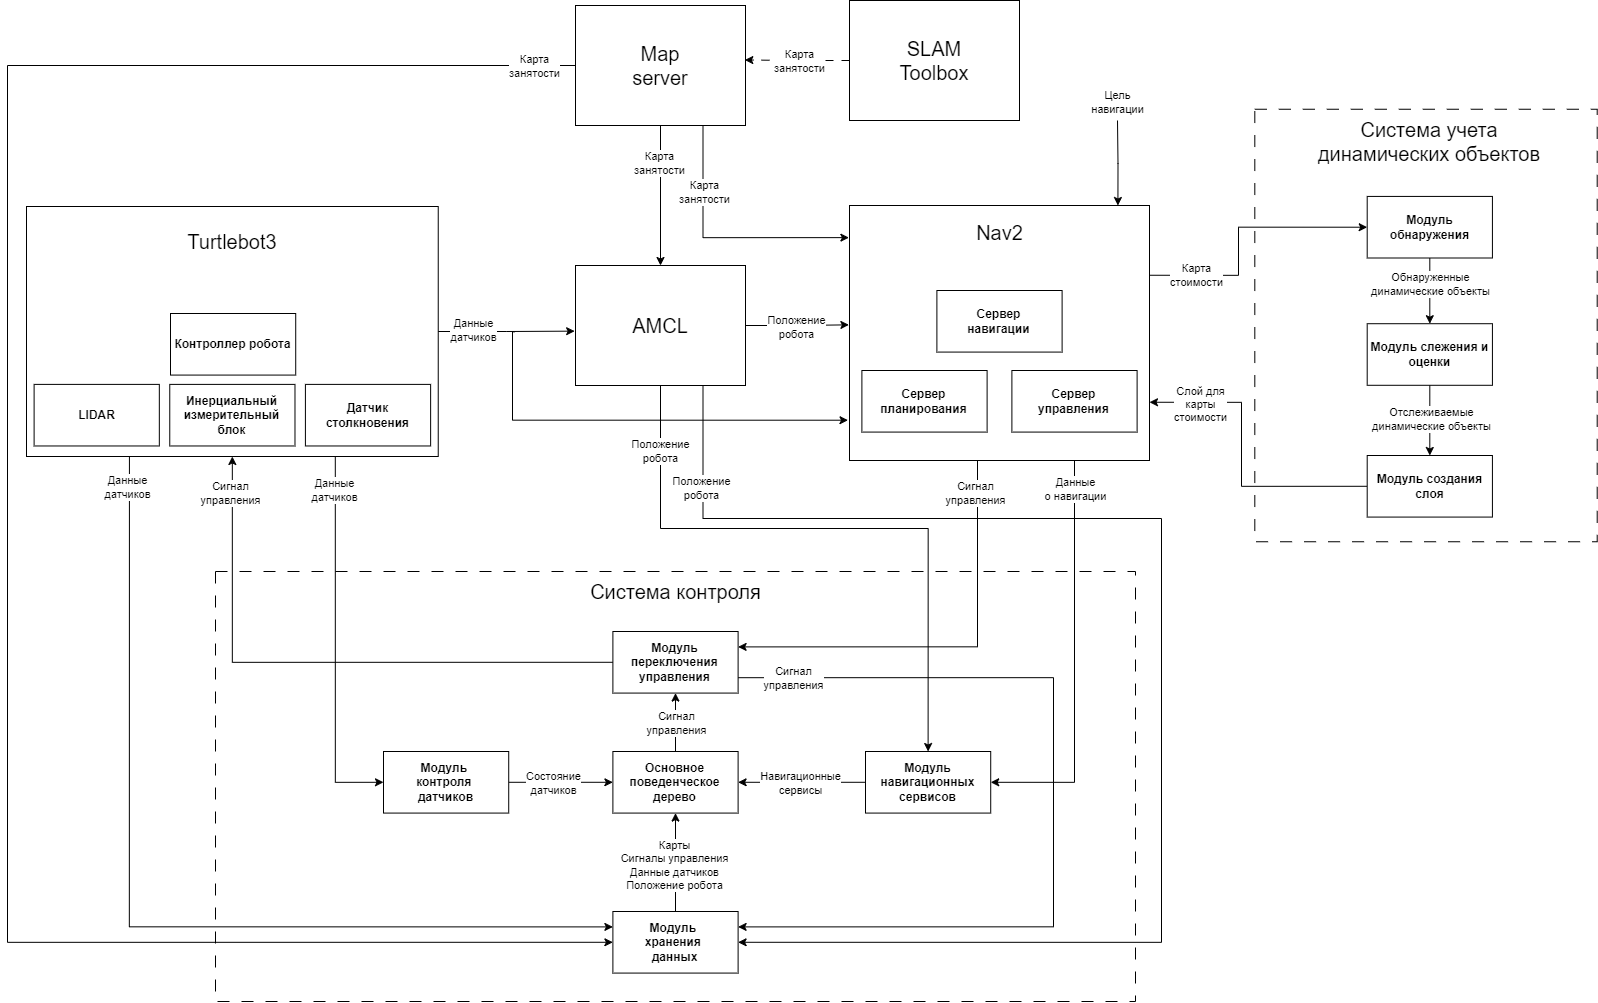
\includegraphics[width=1.0\textwidth]{images/chap_3/full-system.drawio.png}
    \caption{Архитектура системы принятия решений}
    \label{fig:full-system}
\end{figure}

\endinput